\documentclass[../ppG48.tex]{subfiles}
\begin{document}
All the following benchmarks were conducted on a local machine running Ubuntu 22.04 LTS with a 6-core, 12-thread CPU and 32GB of RAM. All tests were conducted on the OpenJDK VM Corretto 21. The JVM was configured with a minimum heap size of 1024MB and a maximum heap size of 16GB.
In the final version of the report, the tests will be conducted on a GitHub-hosted virtual machine under GitHub Actions, running on 4 cores and 8 threads with 16GB of RAM.

For both the Apache Bench and JMeter tests, we simulate a 1000-request warmup period for each route with a concurrent user load of 32 users. The warmup period is followed by the actual test period, during which we simulate 256 requests per user, scaling in increments up to 128 concurrent users.
\subsection{Presentations Results}

\begin{figure}[h]
\centering 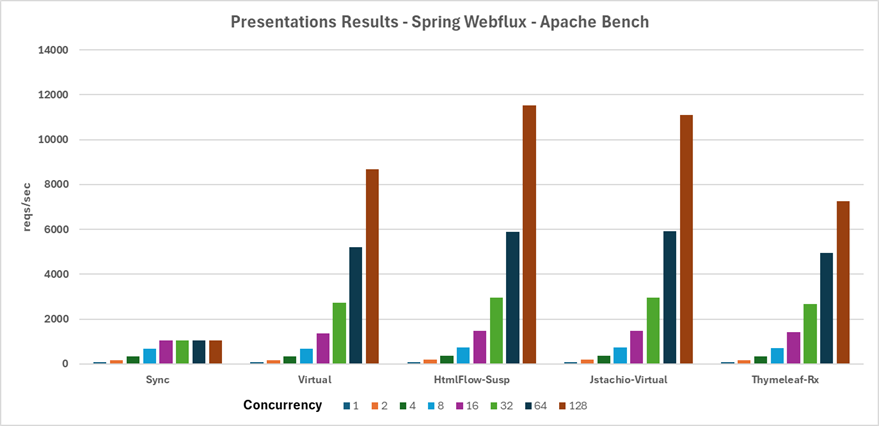
\includegraphics[width=0.8\textwidth]{../Graphs/presentations-webflux-ab.png} \caption{Presentation Benchmark Results in Spring WebFlux with Apache Bench} \label{fig:presentations-webflux-ab} \end{figure}

\begin{figure}[h] \centering 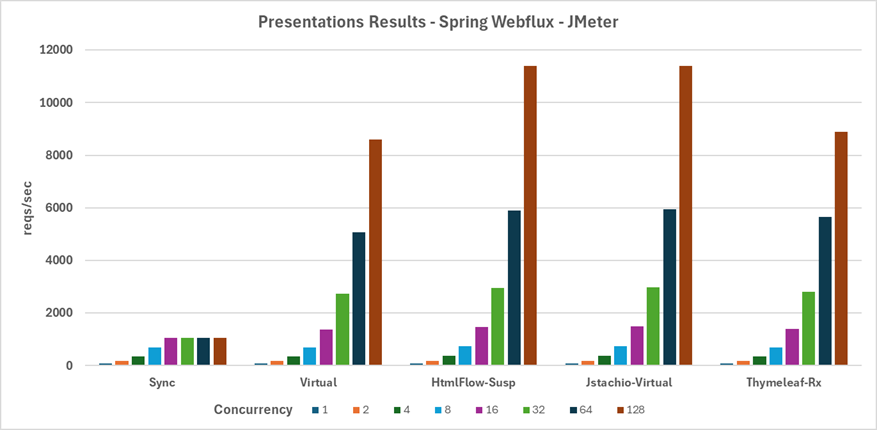
\includegraphics[width=0.8\textwidth]{../Graphs/presentations-webflux-jmeter.png} \caption{Presentation Benchmark Results in Spring WebFlux with JMeter} \label{fig:presentations-webflux-jmeter} \end{figure}

The results in Figures \ref{fig:presentations-webflux-ab} and \ref{fig:presentations-webflux-jmeter} depict the throughput (number of requests per second) for each template engine, with concurrent users ranging from 1 to 128, from left to right. The benchmarks include HtmlFlow using suspendable web templates (HtmlFlow-Susp), Jstachio using Virtual Threads (Jstachio-Virtual), and Thymeleaf using the reactive View Resolver driver (Thymeleaf-Rx). "Sync" and "Virtual" represent the average throughput of the blocking approaches (i.e., KotlinX, Rocker, Jstachio, Pebble, Freemarker, Trimou, HtmlFlow, and Thymeleaf) when run in the context of a separate coroutine dispatcher or Virtual Threads, respectively.

The results show that when using the blocking template engines with a separate coroutine dispatcher, the engines are unable to scale effectively beyond 16 concurrent users. In contrast, the non-blocking engines scale effectively up to 128 concurrent users, with HtmlFlow achieving approximately 11,000 requests per second. When using the blocking approaches in the context of Virtual Threads (achieving non-blocking I/O), the engines scale effectively up to 128 concurrent users, with Jstachio matching HtmlFlow's performance at approximately 11,000 requests per second. Thymeleaf, using the reactive View Resolver driver, also scales to 128 users, albeit less effectively, achieving around 8,500 requests per second.

Additionally, the results show no significant difference between the JMeter and Apache Bench benchmarks, indicating that both tools effectively measure the throughput of the different implementations.

\begin{figure}[h]
\centering 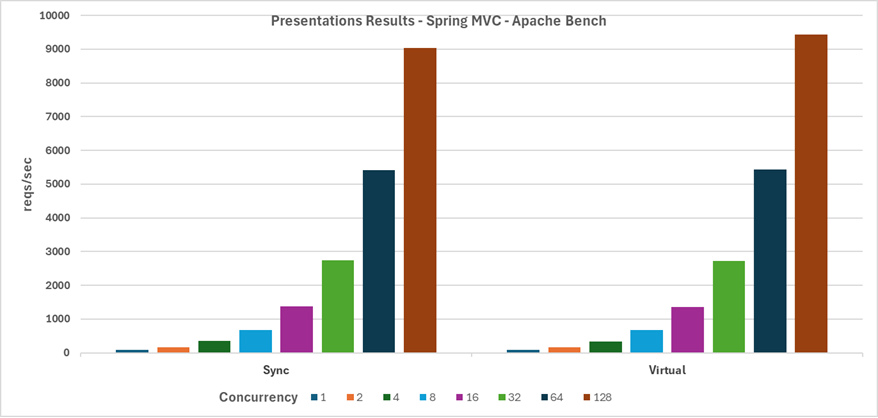
\includegraphics[width=0.8\textwidth]{../Graphs/presentations-springmvc-ab.png} \caption{Presentation Benchmark Results in Spring MVC with Apache Bench} \label{fig:presentations-springmvc-ab} \end{figure}

\begin{figure}[h] \centering 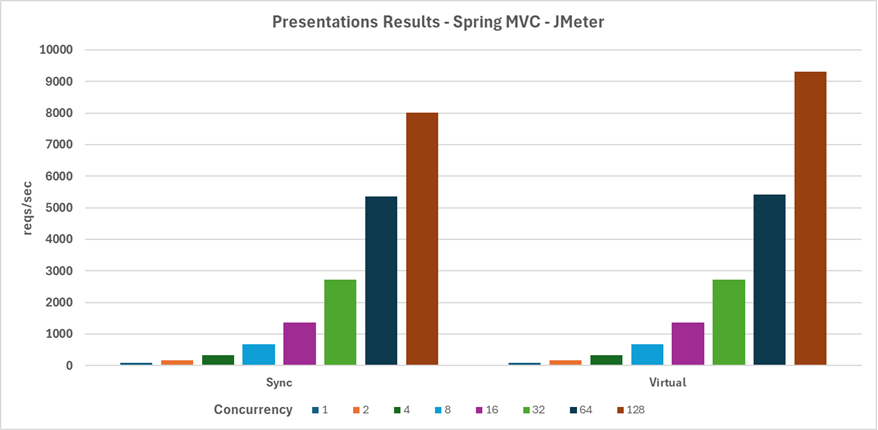
\includegraphics[width=0.8\textwidth]{../Graphs/presentations-springmvc-jmeter.png} \caption{Presentation Benchmark Results in Spring MVC with JMeter} \label{fig:presentations-springmvc-jmeter} \end{figure}

The results for the Spring MVC implementation are shown in Figures \ref{fig:presentations-springmvc-ab} and \ref{fig:presentations-springmvc-jmeter}. "Sync" represents an approach using platform threads with StreamingResponseBody, while "Virtual" uses Virtual Threads.

The results show that both approaches scale effectively up to 128 concurrent users, with the Virtual Thread approach achieving a slightly higher throughput of 9,000 requests per second. These values are slightly lower than those seen in the Spring WebFlux implementation.

There is a slight difference in measured throughput between the JMeter and Apache Bench benchmarks, with Apache Bench achieving a marginally higher throughput for the Sync approach, while the Virtual approach shows similar results across both tools.

\begin{figure}[h]
\centering
 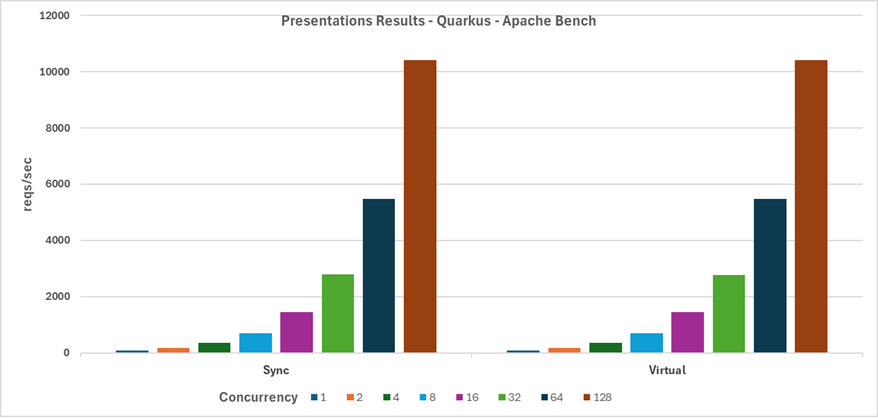
\includegraphics[width=0.8\textwidth]{../Graphs/presentations-quarkus-ab.png} 
 \caption{Presentation Benchmark Results in Quarkus with Apache Bench}
 \label{fig:presentations-quarkus-ab}
\end{figure}

\begin{figure}[h]
     \centering 
     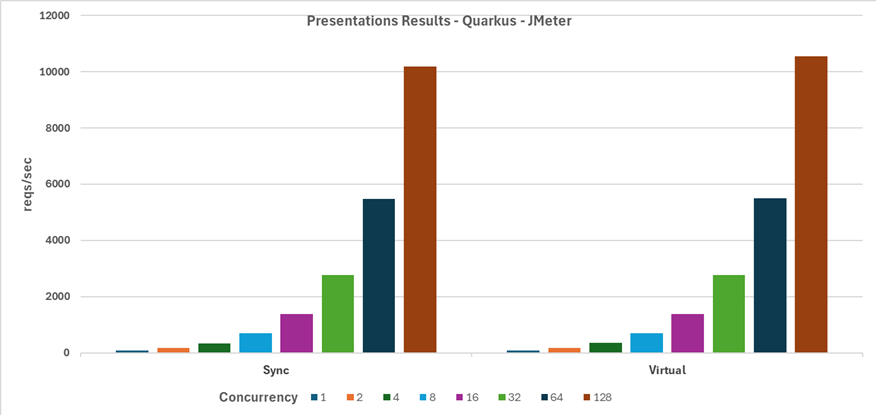
\includegraphics[width=0.8\textwidth]{../Graphs/presentations-quarkus-jmeter.png} 
     \caption{Presentation Benchmark Results in Quarkus with JMeter} 
     \label{fig:presentations-quarkus-jmeter} 
\end{figure}

The results for the Quarkus implementation are shown in Figures \ref{fig:presentations-quarkus-ab} and \ref{fig:presentations-quarkus-jmeter}. "Sync" represents an approach using platform threads with StreamingOutput, while "Virtual" uses Virtual Threads.

The results show that Quarkus handles blocking approaches more effectively than Spring WebFlux, with the blocking engines able to scale up to 128 concurrent users, achieving 10,000 requests per second. Using Virtual Threads results in a slightly higher throughput, but the difference is not significant, with both approaches achieving similar performance.

Again, the difference between the JMeter and Apache Bench benchmarks is negligible.

\subsection{Stocks Results}

\vspace{1cm}

\begin{figure}[h]
\centering 
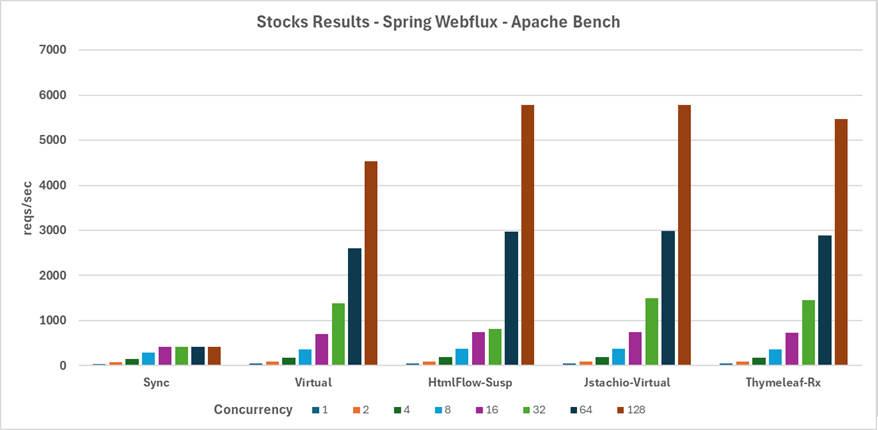
\includegraphics[width=0.8\textwidth]{../Graphs/stocks-webflux-ab.png} 
\caption{Stocks Benchmark Results in Spring WebFlux with Apache Bench}
 \label{fig:stocks-webflux-ab}
\end{figure}

\begin{figure}[h] \centering 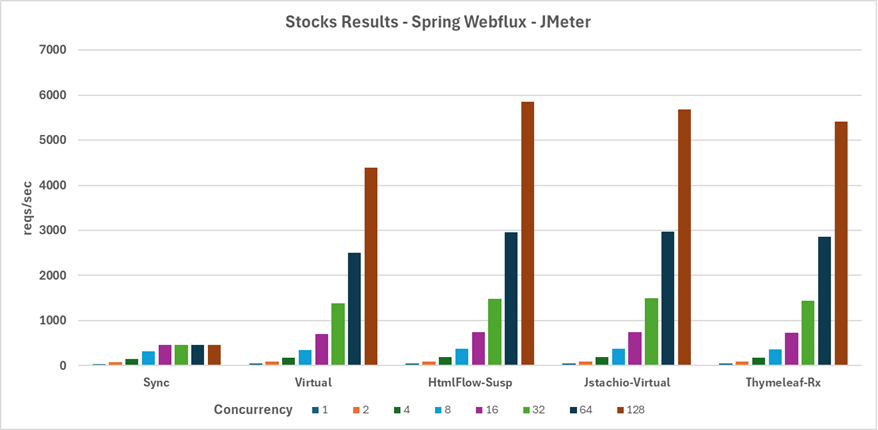
\includegraphics[width=0.8\textwidth]{../Graphs/stocks-webflux-jmeter.png} \caption{Stocks Benchmark Results in Spring WebFlux with JMeter} \label{fig:stocks-webflux-jmeter} \end{figure}

The results in Figures \ref{fig:stocks-webflux-ab} and \ref{fig:stocks-webflux-jmeter} involve the same template engines and approaches as the previous benchmark, but with the data model replaced by the Stock class.

The results show that the scalability of the engines is not significantly affected by the increased complexity of the data model or the increased number of instances (20 instances of the Stock class). However, the throughput is reduced by approximately 50 percent for all engines, with HtmlFlow achieving 6,000 requests per second. The Thymeleaf implementation with the reactive View Resolver driver achieves 5,000 requests per second, indicating that there isn’t a significant performance drop compared to the Presentation benchmark.

JMeter and Apache Bench benchmarks, once again, show similar results.

\begin{figure}[h]
    \centering
    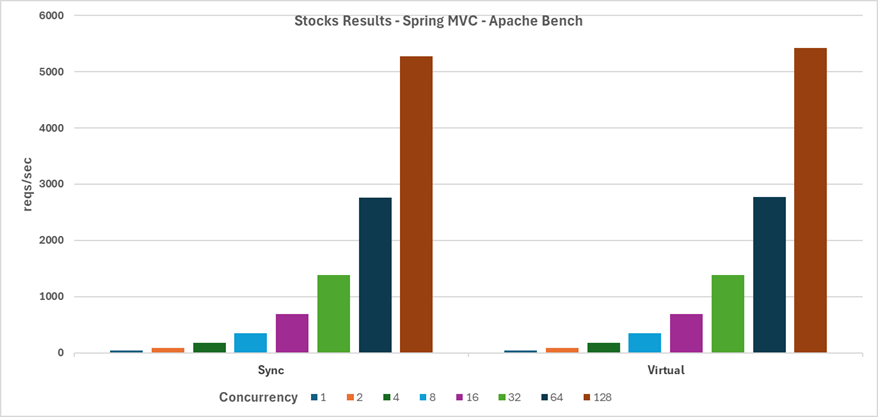
\includegraphics[width=0.8\textwidth]{../Graphs/stocks-springmvc-ab.png} 
    \caption{Stocks Benchmark Results in Spring MVC with Apache Bench}
    \label{fig:stocks-springmvc-ab} 
\end{figure}

\begin{figure}[h] \centering 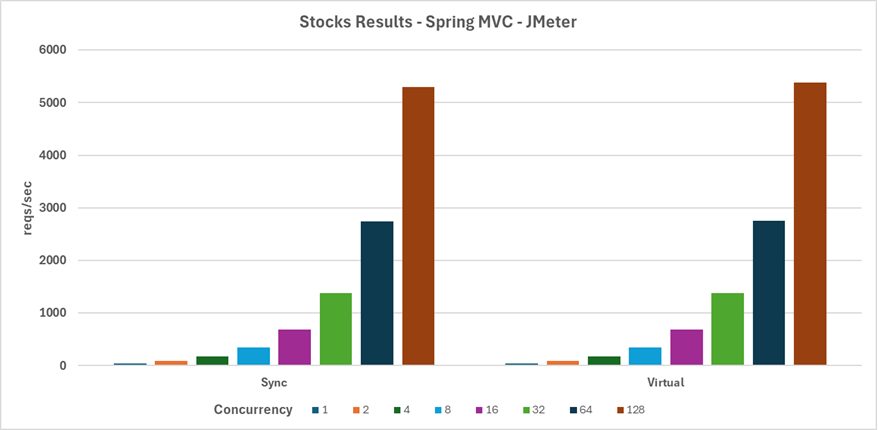
\includegraphics[width=0.8\textwidth]{../Graphs/stocks-springmvc-jmeter.png} \caption{Stocks Benchmark Results in Spring MVC with JMeter} \label{fig:stocks-springmvc-jmeter} \end{figure}

\vspace{4cm}

The results for the Spring MVC implementation are shown in Figures \ref{fig:stocks-springmvc-ab} and \ref{fig:stocks-springmvc-jmeter}. 

The results indicate that for the Stock data model, both approaches scale effectively up to 128 concurrent users, with similar performance outcomes.

\begin{figure}[hbt!]
\centering 
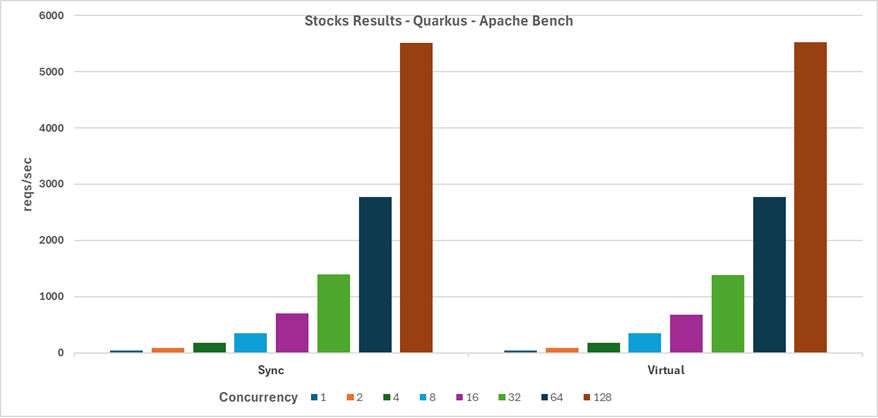
\includegraphics[width=0.8\textwidth]{../Graphs/stocks-quarkus-ab.png}
 \caption{Stocks Benchmark Results in Quarkus with Apache Bench}
  \label{fig:stocks-quarkus-ab} 
\end{figure}

\begin{figure}[hbt!]
     \centering 
     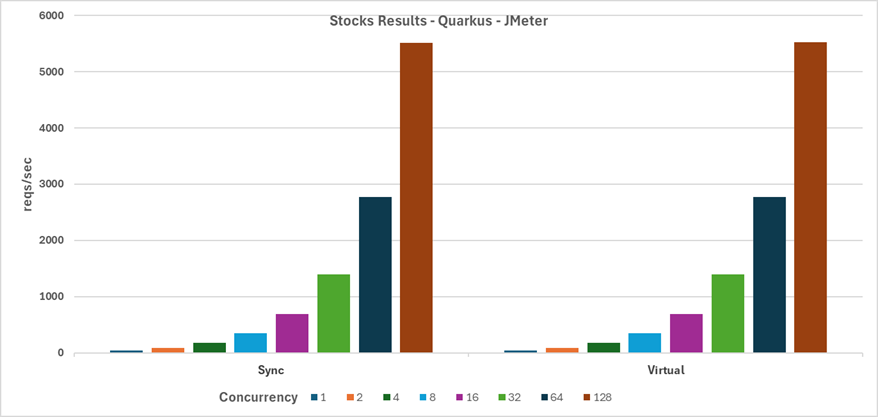
\includegraphics[width=0.8\textwidth]{../Graphs/stocks-quarkus-jmeter.png} 
     \caption{Stocks Benchmark Results in Quarkus with JMeter}
     \label{fig:stocks-quarkus-jmeter}
\end{figure}

\vspace{2cm}

The results depicted in Figures \ref{fig:stocks-quarkus-ab} and \ref{fig:stocks-quarkus-jmeter} show that the Quarkus implementation scales effectively up to 128 concurrent users, achieving performance comparable to the Spring WebFlux implementation. The blocking engines reach 6,000 requests per second. Again, there is no significant difference between the Virtual Threads and platform threads approaches, with both achieving similar results

\end{document}